\chapter{序論}
\thispagestyle{empty}
\label{ch:Introduction}
\minitoc


\newpage

%%=========================================================================================
\section{背景}\label{sec:Background}

% 最初に,章・節・項全体の内容を示す一文を入れ,そこで何の内容を述べるか読者に知らせ,準備してもらう

地震や噴火,豪雨などの自然災害はいつどこで発生するか分からず,誰もがその被害にさらされる可能性がある.
従って,自然災害の発生に備えると共に,その発生後にどのように対処するかは非常に重要である.% "そのため"は口語的,"よって"はより強く後の文章を印象図づける
特に日本は,世界のなかでも自然災害の発生頻度が高いことが知られている.
例えば地震については,日本は地震の震源が集中するプレートの境界線上に位置しており,
内閣府によると,2000年から2009年の間に世界で発生したマグニチュード6.0以上の地震のうち,約20$\%$が日本で発生した\cite{内閣府2010}.
また,日本は活火山の集中する環太平洋造山帯にも位置しているため,世界の活火山のうちの約7.2\%にあたる
111の活火山が日本に分布している\cite{内閣府2010}\cite{気象庁2019a}.
さらに,日本は世界の熱帯低気圧のうち約30\%が発生する北西太平洋に位置し,1970年から2011年にかけて,
年平均約3.8個の台風が上陸した.この上陸数は世界の中では中国,フィリピンに次いで3番目であり,世界各国に上陸する台風の約9.9$\%$に当たる\cite{廣瀬2014}\cite{気象キャスターネットワーク2014}.
このような夏から秋にかけて上陸してくる台風や,春と夏の間に日本に停滞する梅雨前線の影響で,
日本の1年間の降水量は世界平均の約2倍に達している\cite{国交省2004}\cite{気象庁2019b}.
日本と世界におけるマグニチュード6.0以上の地震,活火山,上陸した熱帯低気圧の数を,それぞれ図\ref{fig:num_disaster}(a),(b),および(c)に示す.
% % この後に土砂災害に話がいくようにするには何がより良いか

\begin{figure}[b]
	\begin{center}

		\begin{minipage}[b]{\linewidth}
		\centering
		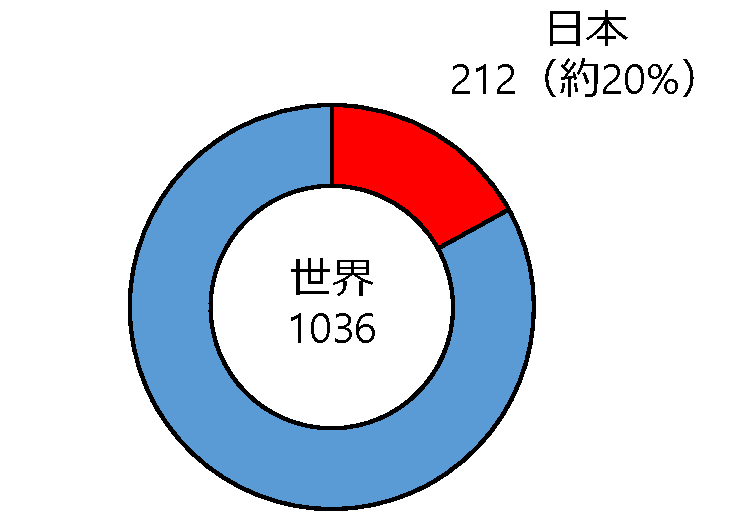
\includegraphics[width=6cm]{./Ch1_Introduction/Fig/num_japan_world_earthquake_compressed.pdf}
		\caption*{(a)マグニチュード6.0以上の地震の発生回数(\cite{内閣府2010}を参考に作成)}
		\end{minipage}

		\vspace{1cm}

		\begin{minipage}[b]{\linewidth}
		\centering
		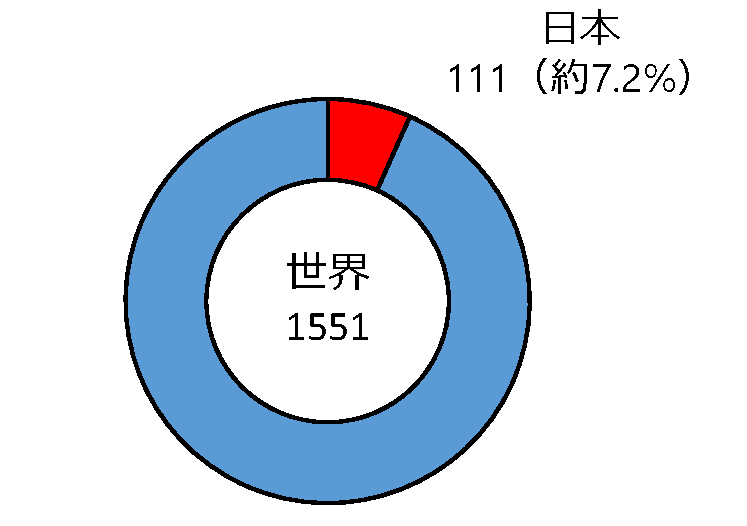
\includegraphics[width=6cm]{./Ch1_Introduction/Fig/num_japan_world_volcano_compressed.pdf}
		\caption*{(b)活火山の数(\cite{内閣府2010}を参考に作成)} 
		\end{minipage}

		\vspace{1cm}

		\begin{minipage}[b]{\linewidth}
		\centering
		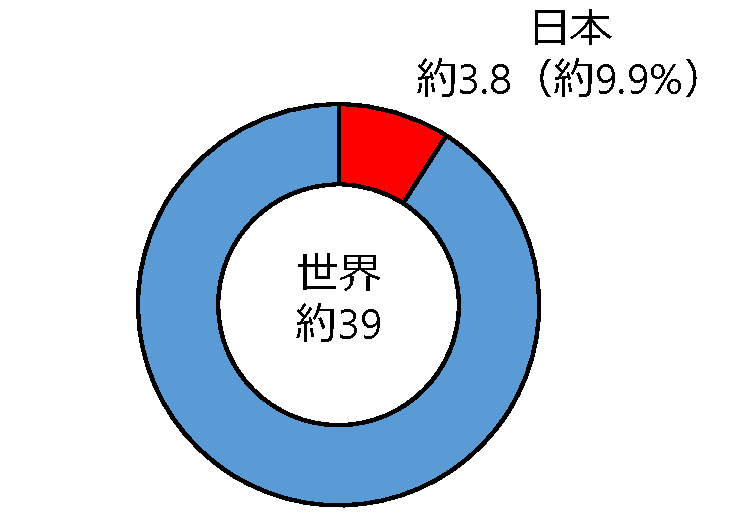
\includegraphics[width=6cm]{./Ch1_Introduction/Fig/num_japan_world_tyhoon_compressed.pdf}
		\caption*{(c)熱帯低気圧の上陸数(\cite{廣瀬2014}を参考に作成)} 
		\end{minipage}
	
	\caption{日本と世界における地震,活火山,上陸した熱帯低気圧の数}\label{fig:num_disaster}
	\end{center}
\end{figure}

\clearpage

% 土砂災害の発生件数が増加
地震,噴火,台風や梅雨前線による豪雨などの大きな自然災害は,土砂災害を誘発することが多い\cite{国交省2007}.
そのため,自然災害の頻発に伴い,土砂災害も多発している.
2008年から2018年の間に発生した土砂災害の件数を図\ref{fig:LandslideN}に示す.
このグラフに示す通り,日本においては,毎年平均1,000件ほどの土砂災害が発生している.
特に2018年には,土砂災害を伴う地震や豪雨などの自然災害が多発したため,
集計開始以降最多の3,459件の土砂災害が発生した.
例えば,2018年9月6日の早朝に発生した北海道胆振東部地震では,震源地となった北海道の胆振地方中東部を中心として広い範囲で,
合計227件の土砂災害が発生した\cite{国交省2019}.
また,2018年の6月28日から7月8日にかけて,停滞していた前線と台風第7号の影響で発生した平成30年7月豪雨でも,
西日本を中心とした全国的に広い範囲で記録的な豪雨となり,合計2,581件の土砂災害が発生した\cite{気象庁2018}.

\begin{figure}[b]
	\begin{center}	
	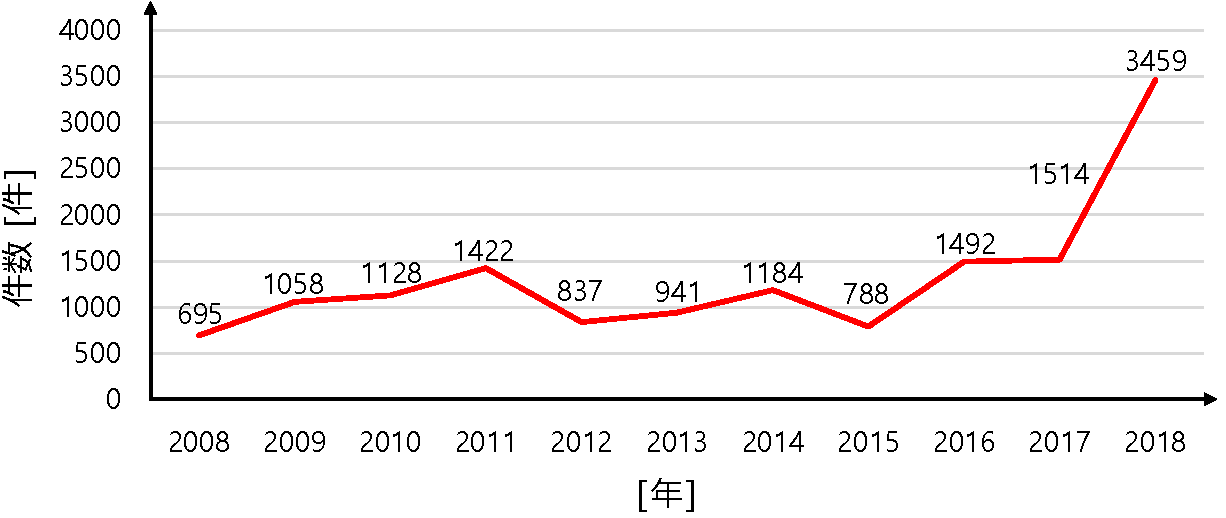
\includegraphics[width=12.5cm]{./Ch1_Introduction/Fig/土砂災害発生件数_compressed.pdf}
	\caption{土砂災害の発生件数(\cite{国交省2019}を参考に作成)}\label{fig:LandslideN}
	\vspace{3cm} % 図を文章のない部分の中心に配置するため
	\end{center}
\end{figure}

\clearpage

% 土砂災害による人的・経済的被害も増加
多発する土砂災害に伴い被害も甚大になっている.
2008年から2018年の間に発生した土砂災害に伴う被害者数と家屋被災戸数を,それぞれ図\ref{fig:LandslideDamage}(a)および(b)に示す.
図\ref{fig:LandslideDamage}(a)および(b)に示す通り,土砂災害の発生件数に比例して被害も増大しており,
2018年には被害者数,家屋被災戸数ともに過去10年間で最大となった.
先ほど言及した北海道胆振東部地震では,土砂災害に伴う死者,負傷者の数が,それぞれ36名,61名に達し,全壊した家屋も44戸に及んだ.
また,平成30年7月豪雨においては,死者,負傷者の数が,それぞれ119名,54名に達し,家屋に対する被害も,全壊364戸,半壊560戸,一部損壊470戸を記録した.
上記の具体例や図\ref{fig:LandslideDamage}(a)および(b)より,土砂災害による人的,経済的被害は無視できないほど甚大になっていることが分かる.

\begin{figure}[b]
	\begin{center}

		\begin{minipage}[b]{\linewidth}
		\centering
		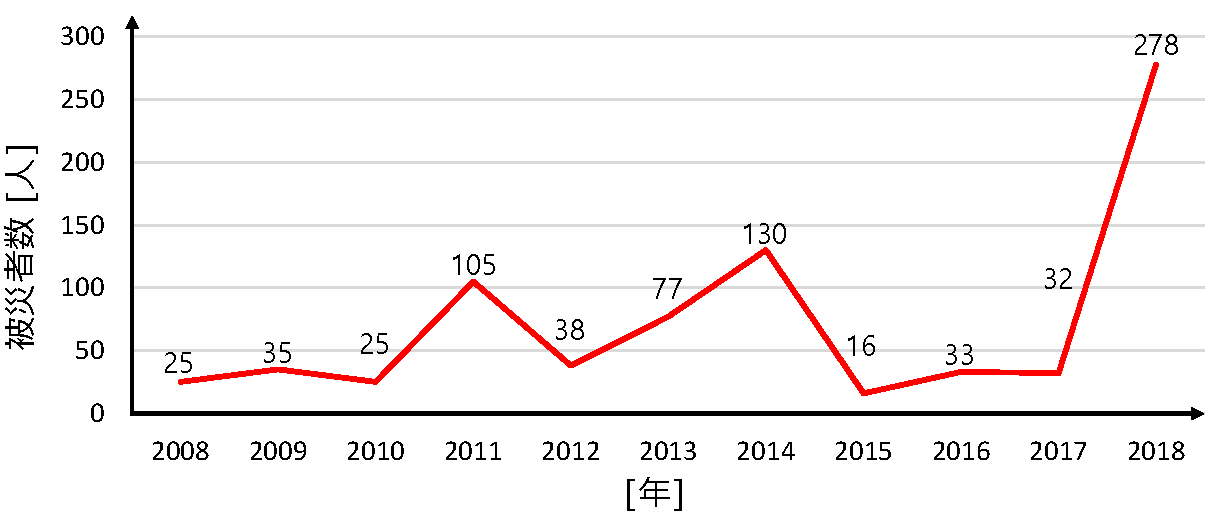
\includegraphics[width=12.5cm]{./Ch1_Introduction/Fig/土砂災害の人的被害_compressed.pdf}
		\vspace{-2mm}
		\caption*{(a)土砂災害の人的被害(死者・行方不明者・負傷者数の合計)} 
		\end{minipage}\\

		\begin{minipage}[b]{\linewidth}
		\centering
		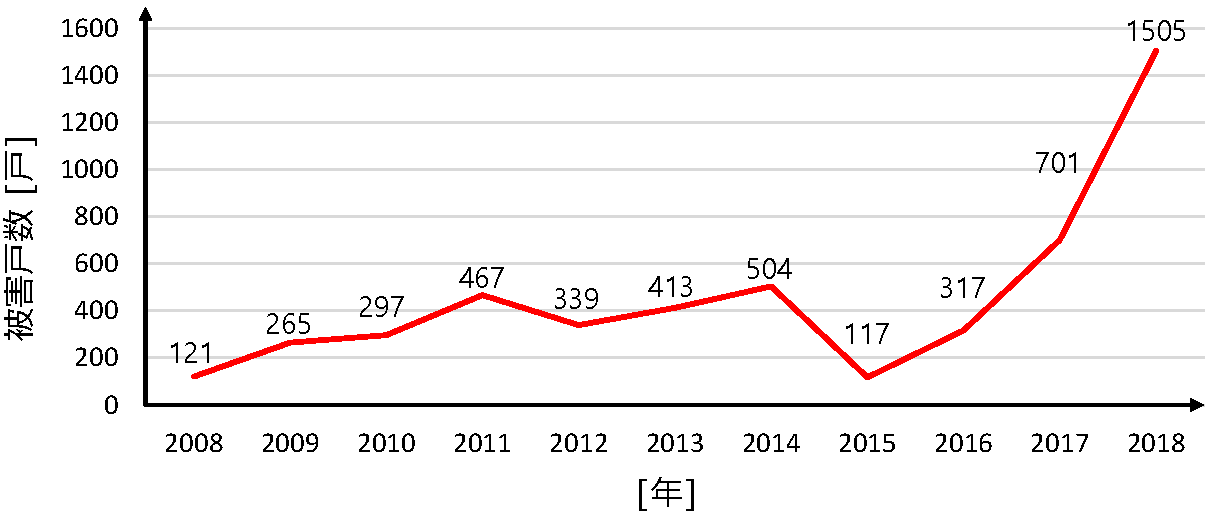
\includegraphics[width=12.5cm]{./Ch1_Introduction/Fig/土砂災害の家屋被害戸数_compressed.pdf}
		\vspace{-2mm}
		\caption*{(b)土砂災害の家屋被害戸数} 
		\end{minipage}
	
	\caption{土砂災害による被害(\cite{国交省2019}を参考に作成)}\label{fig:LandslideDamage}
	\end{center}
\end{figure}

\clearpage

土砂災害による人的,経済的被害を最小限に抑えるためには,
人命救助やライフラインの復旧などを早急に行う必要がある\cite{国交省2016}.
例えば,崩壊してきた土砂や倒壊した家屋の下敷きになった人を救助する場合には,
被災者を3日間以内に救助しなければ,生存率が大幅に低下してしまう\cite{国交省2002}\cite{生田2005}\cite{田畑2006}.
% 阪神淡路大震災の発生時からの経過日数と,救助人数のうちの生存者の割合を示す生存率の関係を図\ref{fig:death_rate_under_house}に示す.
% 図\ref{fig:death_rate_under_house}に示す通り,阪神淡路大震災が発生してから4日以上経過すると,生存率が5\%まで低下することが分かる.
また,電力,水道,通信,道路等のライフラインが土砂災害によって被害を受けた場合,
ライフラインに依存している経済活動も停滞してしまうため,経済的な損失が発生してしまう\cite{豊田2008}\cite{豊田2010}.
従って,人命救助や交通網の確保を早急に行うことは非常に重要であり,
そのためには迅速な復旧工事が必要となる\cite{国交省2016}.
そのために復旧工事において建設機械を使用する必要があるが,
土砂災害の発生した現場の地盤が軟弱な場合,
地盤が建設機械の重量に耐えられずに,建設機械が地盤にはまり込み,最悪の場合転倒する可能性がある\cite{玉手2008}\cite{玉手2014}.
軟弱な地盤にはまり込んだ建設機械を図\ref{fig:sinking_construnction_machine}に示す.
図\ref{fig:sinking_construnction_machine}の画像に示したように建設機械が軟弱な地盤にはまり込むと,
最悪の場合その場で転倒してしまう.
そのような地盤で建設機械を使用することは出来ない.
% 建設機械の使用と建設機械の転倒は直接反するわけではないが,建設機械の転倒から建設機械を使用できないということが伝わるので,"しかし"でOK
従って,復旧工事を行うためには,災害現場において建設機械の走破性を事前に判定することが重要となる.

\begin{figure}[b]
	\begin{center}
	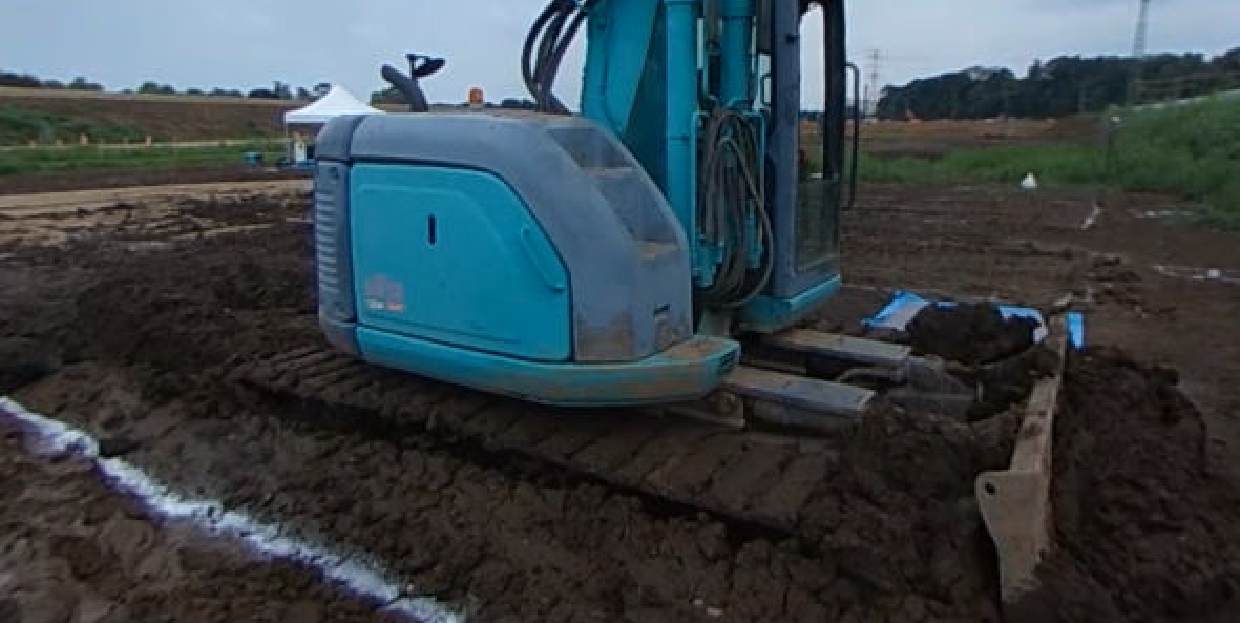
\includegraphics[width=13cm]{./Ch1_Introduction/Fig/trafficability_coneindex_72_72_compressed.pdf}
	\caption{軟弱な地盤にはまり込んだ建設機械(2019年8月28日撮影.詳細は\ref{sec:ConeindexEstimationExperiment}節に記載)}\label{fig:sinking_construnction_machine}
	\vspace{1cm} % 図を文章のない部分の中心に配置するため
	\end{center}
\end{figure}



\clearpage


%%=========================================================================================
\section{先行研究}\label{sec:PreviousStudy}

% 基本的には時制を統一

\subsection{走破性を判定する従来手法}\label{ssec:TraditionalMethod}

建設機械の走破性を判定する従来手法には,走破性の高さを示す指標の1つであるコーン指数を計測する手法がある\cite{Mulqueen1977}\cite{Perumpral1987}.
コーン指数とは,コーンペネトロメータと呼ばれる器具を現場の地面に挿入し,その際に発生する土の抵抗を,% "抵抗力"という言葉はウイルス想起させる
コーンペネトロメータの上部についているダイヤルゲージで読み取ることで得られる値である.
土の抵抗力が強いほど建設機械の走破性が高いので,
コーン指数が高いほど建設機械の走破性が高いと判定できる.
コーンペネトロメータとそれを用いたコーン指数の測定の様子を,それぞれ図\ref{fig:ConeIndexMeasurement}(a)および(b)に示す.
図\ref{fig:ConeIndexMeasurement}に示す通り,これまでコーン指数の測定は人の手で行われてきた.
しかし,災害現場では2次災害の危険が存在するため,
現場で人がコーンペネトロメータを挿入してコーン指数を測定することは大変危険である.
従って,災害現場における建設機械の走破性を判定するためには,
% 無人でコーン指数を測定するすることによって,
遠隔で走破性を判定する必要がある.

\begin{figure}[p]
	\begin{center}
		\begin{tabular}{c} % 隣り合う図がずれないようにする

			\begin{minipage}[b]{0.45\linewidth}
			\centering
			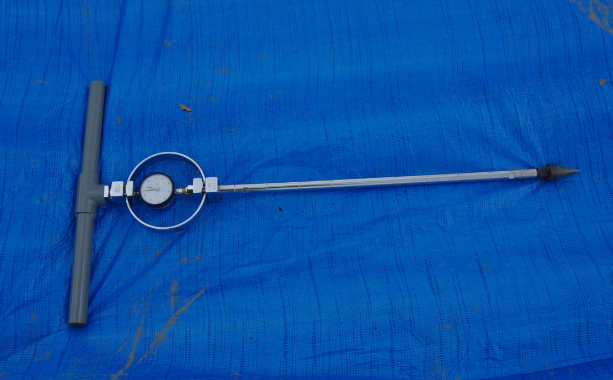
\includegraphics[width=8cm, angle=-90]{./Ch1_Introduction/Fig/コーンペネトロメータa.PNG}
			\setlength{\captionmargin}{30pt}\caption*{(a)コーンペネトロメータ\protect\linebreak(2019年8月28日撮影)}
			\end{minipage}

			\hfill

			\begin{minipage}[b]{0.45\linewidth}
			\centering
			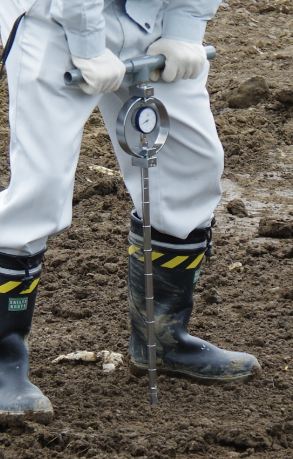
\includegraphics[height=8cm]{./Ch1_Introduction/Fig/コーンペネトロメータb.PNG}
			\setlength{\captionmargin}{20pt}\caption*{(b)コーン指数の測定の様子\protect\linebreak(2019年8月28日撮影)}
			\end{minipage}

		\end{tabular}
	\caption{コーンペネトロメータを用いたコーン指数の測定}\label{fig:ConeIndexMeasurement}
	\end{center}
\end{figure}

\clearpage

\subsection{遠隔で走破性を判定する手法}\label{ssec:UnmannedMethod}

遠隔で走破性を判定するためには,遠隔でコーン指数を測定する必要がある.
遠隔でコーン指数を測定する先行研究には,
% ロボットにコーン指数を測定する器具を搭載し,% "~には"という文言で統一
コーン指数を測定する器具を搭載したロボットを遠隔操作で対象とする環境まで移動させ,搭載した器具でコーン指数を測定する
手法が提案されている\cite{RobotWatch2002}\cite{Zacny2010}\cite{Chhaniyara2012}\cite{古谷2016}.
この手法は,人の手によるコーン指数の測定を,遠隔操作できるロボットに
置き換えることによって遠隔でのコーン指数の測定を達成している.
しかし,コーン指数の測定器具を測定地点に1カ所ずつ接触させる必要があるため,
地盤が軟弱な場合や急勾配の斜面がある場合など,対象とする環境にロボットを移動させることができない場合には,
コーン指数の測定が不可能となるという問題がある.
ロボットを対象とする環境に移動させることができない場合でも
走破性を判定するためには,
% 非接触でのコーン指数推定によって
非接触で走破性を判定する必要がある.

\subsection{非接触で走破性を判定する手法}\label{ssec:NonContactMethod}

非接触で走破性を判定するためには,非接触でコーン指数を推定する必要がある.
非接触でコーン指数を推定する先行研究には,
水が光を吸収する近赤外の波長帯を撮影した画像を用いてコーン指数を推定する手法が提案されている\cite{Rankin2010}\cite{Fernandez2015}.
この手法は,土に含まれる水の量が増加すると,一般的にコーン指数が減少することを利用している.
土に含まれる水の量が増加すると,水は近赤外の光を吸収するため土から反射してくる近赤外の光の強さは減少し,同時にコーン指数も減少する.
従って,土から反射してくる近赤外の光の強さとコーン指数は相関関係にあるため,
土の近赤外の光の強さからコーン指数をある程度推定することができる.
% この手法は,コーン指数が土に含まれる水の量に大きく影響されることと,
% 水が近赤外の光を吸収することを利用し,
% 土中の水の量が増加するのに伴い,土からの近赤外の光の強さは減少し,一般的にはコーン指数が減少するため,
この手法は,近赤外の波長帯を撮影した画像を用いて土からの近赤外の光の強さを測定することによって,非接触でのコーン指数の推定を達成している.
しかし,この手法は,土に含まれる水の量を示す指標である含水比にのみ注目し,
含水比以外でコーン指数に影響を与える土の種類には注目していないため,コーン指数の推定精度が低いという問題がある.

一方,スペクトル画像から得られた分光反射率スペクトルを用いてコーン指数を非接触で推定する手法も提案されている\cite{Kruse2000}\cite{Sopher2016}.
この手法は,コーン指数が土の種類に大きく影響されることと,
土の種類によって分光反射率スペクトルが異なることを利用している.
土の種類ごとにそれぞれ固定の分光反射率スペクトルが存在し,コーン指数も異なるため,
分光反射率スペクトルからコーン指数をある程度推定することができる.
しかし,この手法のように,固定された分光反射率スペクトルを用いて物質の種類を識別する際には,
外部の状況によって左右されない分光反射率スペクトルを用いるため,
土に含まれる水の量などの外部の状況によって変動する部分の分光反射率スペクトルは使用されない\cite{Shaw2003}.
この手法においても,水が光を吸収するため水の量によって変動する近赤外の分光反射率スペクトルは使用されていない.
従って,
% この手法は水が光を吸収する波長帯を除いた分光反射率スペクトルを用いてコーン指数を推定しているため,% 同じこと言っている
結果的に土の種類にのみ注目し,
含水比には注目していないことになる.
よって,この手法においてもコーン指数の推定精度が低いという問題が残る.

\ref{ssec:TraditionalMethod}項,\ref{ssec:UnmannedMethod}項,およびこの\ref{ssec:NonContactMethod}項で
解説した,コーン指数に基づく走破性の判定手法とその特徴を,表\ref{tbl:traditional_and_previous_method}に示す.
% 表\ref{tbl:traditional_and_previous_method}において,左の列から順に,\ref{ssec:TraditionalMethod}項,\ref{ssec:UnmannedMethod}項,
% \ref{ssec:NonContactMethod}項で解説した手法の,それぞれの場合における
表\ref{tbl:traditional_and_previous_method}より,\ref{ssec:TraditionalMethod}項や\ref{ssec:UnmannedMethod}項で
解説した手法では,土砂災害の発生現場で考慮する必要のある,2次災害や,軟弱または急勾配な地盤に対応できないため,
土砂災害の発生現場で使用するには不適切である.一方,2次災害や,軟弱または急勾配な地盤に対応できる\ref{ssec:NonContactMethod}項で
解説した手法では,コーン指数の推定精度が低いという問題がある.
そこで,土砂災害の発生現場で高精度な走破性判定を行うためには,この\ref{ssec:NonContactMethod}項で
解説した,画像を用いたコーン指数の推定において,コーン指数の推定精度を向上させる必要があることが分かる.
% 上記に示した通り,画像を用いてコーン指数を推定する
先ほど解説した通り,画像を用いてコーン指数を推定する先行研究では,コーン指数に大きく影響する土の種類と含水比のどちらか一方のみに
注目した手法が目立つ.
そこで,先行研究よりもコーン指数推定の精度を向上させるためには,土の種類と含水比の双方に注目する必要がある.

\begin{figure}[b]
	\begin{center}
	\tblcaption{走破性を判定するための従来手法と先行研究の特徴}\label{tbl:traditional_and_previous_method}
	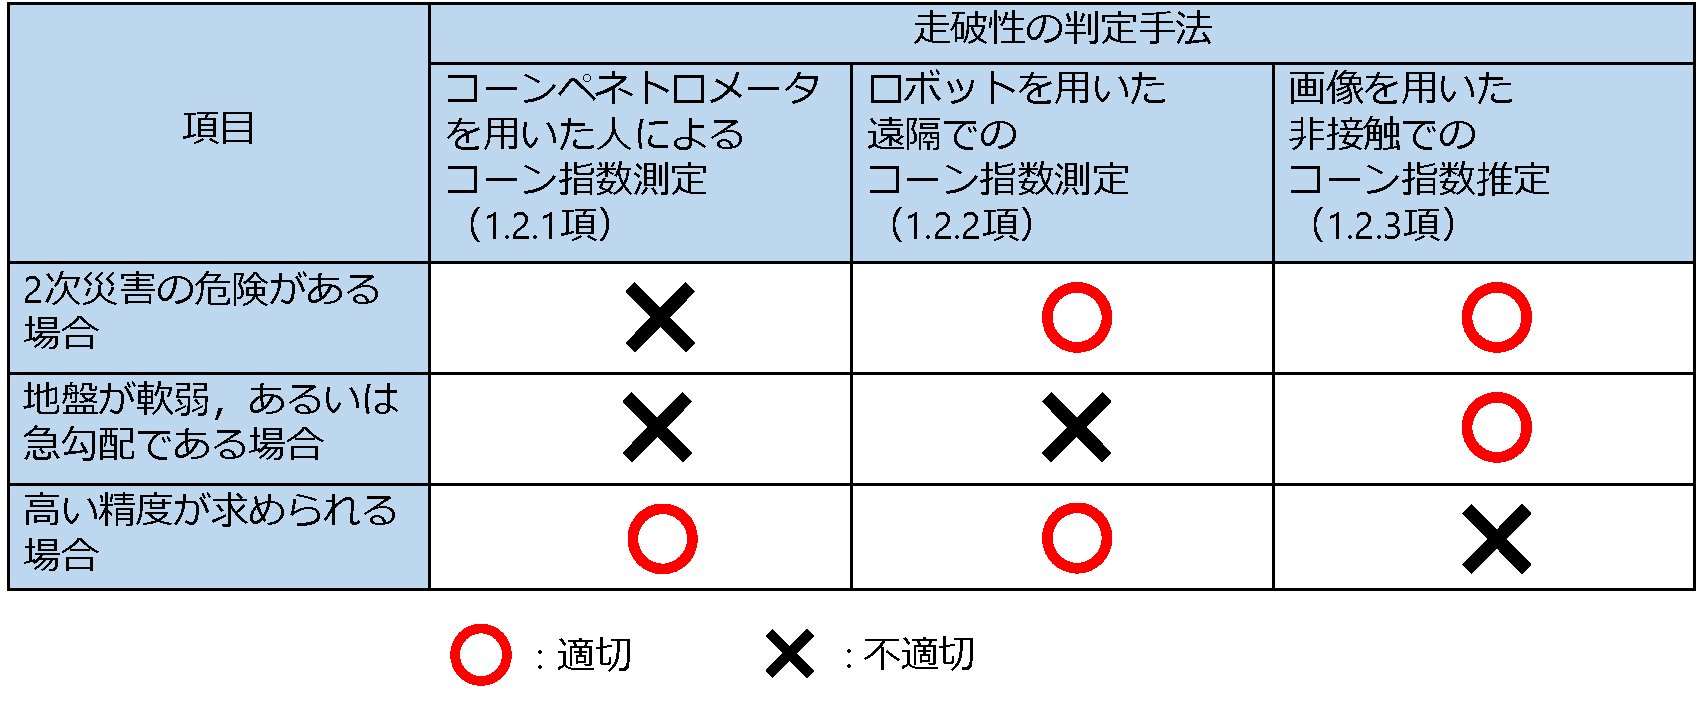
\includegraphics[width=13cm]{./Ch1_Introduction/Fig/traditional_and_previous_method_compressed.pdf}
	\vspace{1cm} % 図を文章のない部分の中心に配置するため
	\end{center}
\end{figure}

\clearpage


%%=========================================================================================
\section{本研究の目的}\label{sec:Objective}

\ref{sec:Background}節において,土砂災害が発生した災害現場では,建設機械を使用する前に走破性を判定する必要があることを述べた.
次に,\ref{sec:PreviousStudy}節において,災害現場での走破性の判定には,
非接触での走破性判定が求められており,
そのために非接触でコーン指数を推定する必要があることを述べた.
また,コーン指数には土の種類と含水比の双方が大きく影響しているため,双方に注目する必要があるが,
従来の非接触でコーン指数を推定する手法には,双方に注目した手法が確認されていないことにも言及した.
そこで,本研究の目的を以下の通りとする.

\vspace{5pt}
\begin{itembox}[c]{目的}
\begin{center}
土の種類と含水比の双方に注目した\\非接触での建設機械のための走破性判定
\end{center}
\end{itembox}
\vspace{5pt}

% 提案手法の概要
本研究においては,まず非接触で土の種類の識別と含水比の推定を行い,
それらを用いてコーン指数を推定することによって,非接触での走破性判定を行う.
また,土の種類の識別と含水比の推定を非接触で行うために,
スペクトル画像という画像を用い,そこから取得する分光反射率スペクトルを用いる.

\clearpage

%%=========================================================================================
\section{本論文の構成}\label{sec:Structure}

本論文は,全6章から構成されている.
本論文の構成を\mbox{図\ref{fig:MThesisConstitution}}に示す.

第\ref{ch:Introduction}章では,土砂災害の発生現場における建設機械の走破性の判定の必要性と,
そのために非接触での走破性判定が必要であることを述べた.
従来の非接触での走破性判定においては,走破性を示す指標の1つであるコーン指数を非接触で推定していた.
しかし,その手法では,コーン指数に大きな影響を与える
土の種類と含水比の双方に注目した手法は確認されていないことにも言及した.
そこで,本研究における目的を,土の種類と含水比の双方に注目した非接触での走破性判定とすることを述べた.
そのために,スペクトル画像から取得する分光反射率スペクトルを用いて
土の種類の識別と含水比の推定を行い,その2つからコーン指数を推定するという提案手法について簡単に解説した.
% 非接触での走破性判定:目的
% 画像を用いたコーン指数の推定:手段
% "実施"ではなく"行う"という文言に統一

第\ref{ch:PrinciplesOfMethod}章では,
非接触での走破性判定のために本研究で提案した,
スペクトル画像から土の種類の識別と含水比の推定を行い,その2つを用いてコーン指数を
推定する手法で利用する原理について述べる.
まず,分光反射率スペクトルを用いた土の種類の識別と含水比の推定で利用する原理と,
その土の種類と含水比からコーン指数を推定する際に利用する原理の2つについて解説する.% "~の原理"という用例が多い
次に,分光反射率スペクトルを取得するスペクトル画像について述べる.% "~について述べる"という用例で基本的には統一
最後に,スペクトル画像を用いて推定したコーン指数による,
非接触での走破性判定の有効性について議論する.

第\ref{ch:SoilTypeDiscrimination}章では,
非接触での走破性判定のために本研究で提案した手法の最初のステップである,
スペクトル画像を用いて土の種類を識別するステップの詳細について述べる.
まず,本研究では,土の種類ごとに分光反射率スペクトルが異なることを利用し,
スペクトル画像から取得した分光反射率スペクトルを用いて土の種類を識別することを述べる.
次に,多くの土の種類を分光反射率スペクトルから識別するためには,
% 波長分解能の高い
非常に多くの波長帯の光の強さを記録する分光反射率スペクトルを取得する必要があることに言及し,
それを取得するためには,入射光を分光させてその強さを記録した波長帯の幅を狭くした,
波長分解能の高いスペクトル画像が必要となることを述べる.
% 土の種類を識別するためには波長分解能の高い詳細な分光反射率スペクトルを取得する必要がある.
そのために,本研究では,一般的なRGB画像が取得するR,G,Bの3波長帯以外の波長帯も取得するマルチスペクトル画像のなかでも,
波長分解能の高いマルチスペクトル画像を土の種類の識別に使用することを述べる.
最後に,上記で解説した,スペクトル画像を用いて土の種類を識別するステップの有効性を確認するために実施した
検証実験とその結果について解説と考察を行う.

第\ref{ch:WaterContentEstimation}章では,
非接触での走破性判定のために本研究で提案した手法の2番目のステップである,
スペクトル画像を用いて含水比を推定するステップの詳細について述べる.
まず,本研究では,水が近赤外の光を吸収することを利用し,
スペクトル画像から取得した近赤外の波長帯と水が光を吸収しない波長帯の,2つの波長帯の分光反射率の差を用いて% "水が光を吸収する・しない"という用例で基本的には統一し,"吸光波長帯"という単語は使用しない.
含水比を推定することを述べる.
次に,水は近赤外の広い範囲の光を吸収するため,近赤外の広い範囲を1つの波長帯で取得する必要があることに言及し,
近赤外の広い範囲を1つの波長帯で取得するためには,幅が広い波長帯を取得できるようにしたスペクトル画像が必要となることを述べる.
そのために,本研究では,スペクトル画像のなかでも,
光の強さを記録する波長帯の数が比較的少数である代わりに,1つ1つの波長帯の幅を広くとることができるため,
近赤外の広い範囲を1つの波長帯で取得できる
マルチスペクトル画像を使用することを述べる.
最後に,上記で解説した,スペクトル画像を用いて含水比を推定するステップの有効性を確認するために実施した
検証実験とその結果について解説と考察を行う.

第\ref{ch:ConeIndexEstimation}章では,
非接触での走破性判定のために本研究で提案した手法の最後のステップである,
識別した土の種類と推定した含水比からコーン指数を推定するステップの詳細について述べる.
まず,本研究では,土の種類と含水比が分かればコーン指数が推定可能であることを利用し,
第\ref{ch:SoilTypeDiscrimination}章で識別した土の種類と
第\ref{ch:WaterContentEstimation}章で推定した含水比から
コーン指数を推定することを述べる.
次に,土の種類と含水比からコーン指数を推定するためには,土の種類ごとの含水比とコーン指数の関係を予め把握する必要があることに言及し,% "含水比","コーン指数"という順番
そのために,予め土の種類ごとに含水比を変えてコーン指数を測定し,
土の種類によって異なる含水比とコーン指数の関係を記録することを述べる.
最後に,上記で解説した,識別した土の種類と推定した含水比からコーン指数を推定するステップの有効性を確認するために
屋外の工事現場で実施した検証実験とその結果について解説と考察を行う.

第\ref{ch:Conclusion}章では,本論文の結論と今後の展望を述べる.

\begin{figure}[p]
	\begin{center}
	\centering
	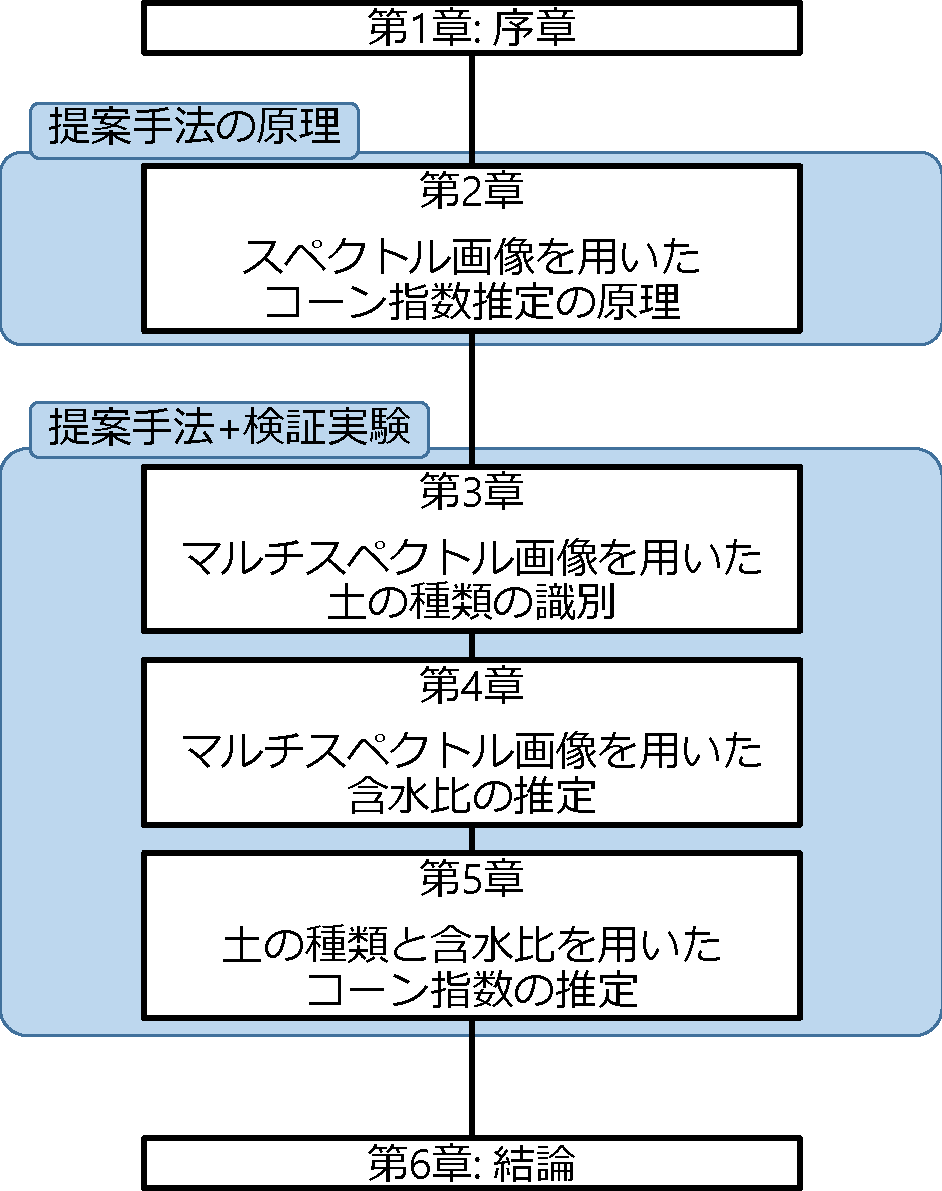
\includegraphics[width=8cm]{./Ch1_Introduction/Fig/thesis_constitution_compressed.pdf}
	\caption{修論構成}\label{fig:MThesisConstitution}
	\end{center}
\end{figure}

\clearpage


%%%本文終了